\documentclass[tikz,border=3pt]{standalone}
\usepackage[T1]{fontenc}
\usepackage{mathptmx}
\usepackage{tikz,pgfplots}
\usetikzlibrary{arrows.meta,positioning,calc,fit,backgrounds,shapes.geometric}
\pgfplotsset{compat=1.18}
\definecolor{forest}{HTML}{346E57}
\definecolor{sage}{HTML}{E8EFEA}
\definecolor{clay}{HTML}{AC653F}
\definecolor{sand}{HTML}{F4EAE2}
\definecolor{ink}{HTML}{252525}
\definecolor{light}{HTML}{F5F5F3}
\definecolor{gridgray}{HTML}{D8DAD6}
\tikzset{box/.style={draw=ink!70,line width=.5pt,rectangle,rounded corners=1pt,fill=white,align=center,font=\fontsize{11}{12}\selectfont,inner sep=6pt}, flow/.style={-{Latex[length=2.4mm]},line width=.7pt,draw=ink!80}, data/.style={flow,densely dashed,draw=forest}, label/.style={font=\fontsize{10}{11}\selectfont,fill=white,inner sep=2pt,align=center}}
\hyphenpenalty=10000\exhyphenpenalty=10000\begin{document}
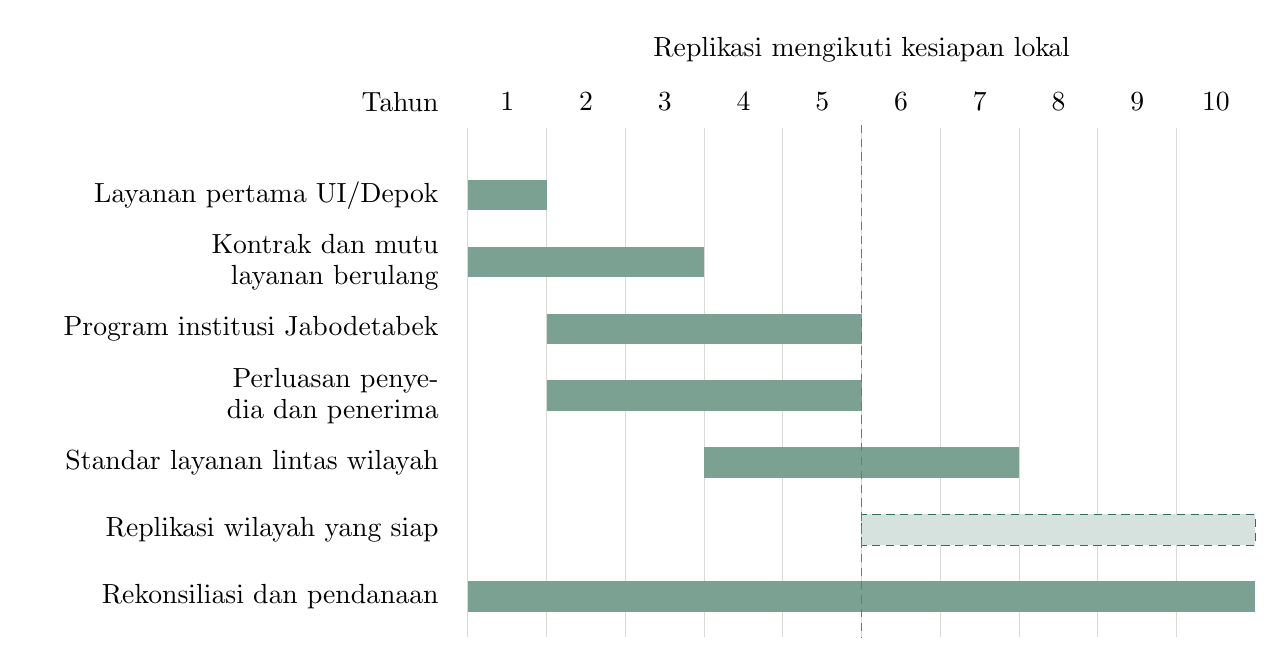
\begin{tikzpicture}[x=1cm,y=.85cm]
\foreach\y in{1,...,10}{\draw[gridgray,line width=.35pt](\y,0)--(\y,-7.6);\node[font=\fontsize{10}{11}\selectfont]at(\y+.5,.4){\y};}
\node[anchor=east,font=\fontsize{10}{11}\selectfont]at(.75,.4){Tahun};
\foreach\r/\s/\e/\lab in{1/1/1/{Layanan pertama UI/Depok},2/1/3/{Kontrak dan mutu layanan berulang},3/2/5/{Program institusi Jabodetabek},4/2/5/{Perluasan penyedia dan penerima},5/4/7/{Standar layanan lintas wilayah},6/6/10/{Replikasi wilayah yang siap},7/1/10/{Rekonsiliasi dan pendanaan}}{
\node[anchor=east,text width=5.1cm,align=right,font=\fontsize{10}{11}\selectfont]at(.75,-\r){\lab};
\ifnum\s>5\fill[forest!20](\s,-\r-.23)rectangle(\e+1,-\r+.23);\draw[forest,densely dashed](\s,-\r-.23)rectangle(\e+1,-\r+.23);\else\fill[forest!65](\s,-\r-.23)rectangle(\e+1,-\r+.23);\fi}
\draw[clay,densely dashed](6,.05)--(6,-7.6);
\node[font=\fontsize{10}{11}\selectfont,anchor=south]at(6,.85){Replikasi mengikuti kesiapan lokal};
\end{tikzpicture}
\end{document}
